Альтернативным путем является подход байесовской оценки знания,
описанный в работе \cite{corbett1994knowledge}


\begin{figure}[h]
    \centering
    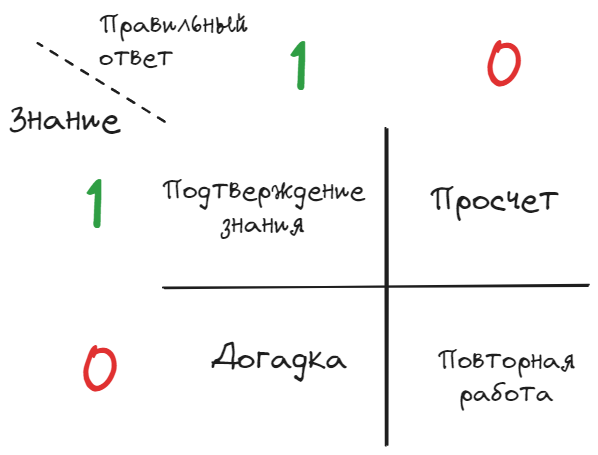
\includegraphics[width=0.5\textwidth]{assets/work/rating/bkt.excalidraw.png}
    \caption{Матрица исходов модели Байесовской оценки на шаге t}
    \label{bkt}
\end{figure}

Задача модели подобрать три ключевых параметра \begin{itemize}
    \item $P(L_0)$ начальные знания в предмете
    \item $P(S) = P(x=0| L_t = 1)$ вероятность просчета при наличи знаний
    \item  $P(G) = P(x=1| L_t = 1)$ вероятность угадать при отсутствии знаний
\end{itemize}

При их подборе Байесов подход к оценке
позволяет обновлять представления о
степени знаний согласно правилам

$$  
    P(L_t| obs_t=1) = \frac{P(L_t)(1-P(S)}{P(L_t)(1-P(S)) + (1-P(L_t))P(G))} \\
    P(L_t| obs_t=0) = \frac{P(L_t)P(S)}{P(L_t)(1-P(S)) + (1-P(L_t))P(G))} 
$$

\textit{Лемма} Доказательства вида апостериорного
 пересчета.
\textit{Доказательство}\qed
Сопряженным к биномальному множеству
является бета распределение 

Модель предполагает, что вероятность забыть $ P(L_{t+1}=0|L_t=1)=0$

\blacksquare